\documentclass[a4paper]{article}

\usepackage[english]{babel}
\usepackage[utf8]{inputenc}
\usepackage{amsmath}
\usepackage{graphicx}
\usepackage[colorinlistoftodos]{todonotes}
\usepackage{float}

\title{CMSI 370 Music Project}

\author{Joseph Barbosa}

\date{September 25, 2014}

\begin{document}
\maketitle

\begin{abstract}
During our Interaction Design course we have gone over such elements as usability measurements and guidelines documents without doing testing of our own. This assignment was meant just for that, we were to test out two rival platforms and analyze the results. For our specific platforms we chose two Music Apps, Spotify and Itunes, and we were able to test how well the apps complied to their guidelines documents through field testing. We were able to base our analysis on the usability metrics of efficiency, errors, and satisfaction and we found that Spotify tested superior to itunes. Based on our results, Spotify tends to adhere to its guidelines documents more accurately and it exceeded the marks set by itunes in our testing of the three usability metrics.
\end{abstract}

\section{Introduction}

In conducting our field tests for this assignment, we asked several users to completet three tasks which were determined by our team to test the compliance of the apps to their guidelines documents. The first of the three tasks was for the user to begin from the main library of each platform and from there create a new playlist with the title "Hello World". The second was for the user to create and start a "Tiesto" radio station, starting from the main library. Lastly, our third task was to choose a specific playlist which has been previously filled, from the main library, enter it, and set it to repeat indefinitely. In the next section I will be listing our results from the field tests for each task and how they compare. The order of importance for our usability measurements goes from greatest to least as follows: efficiency, errors, satisfaction.



\section{Tasks}
\label{sec:tasks}

\begin{figure}[H]
\centering
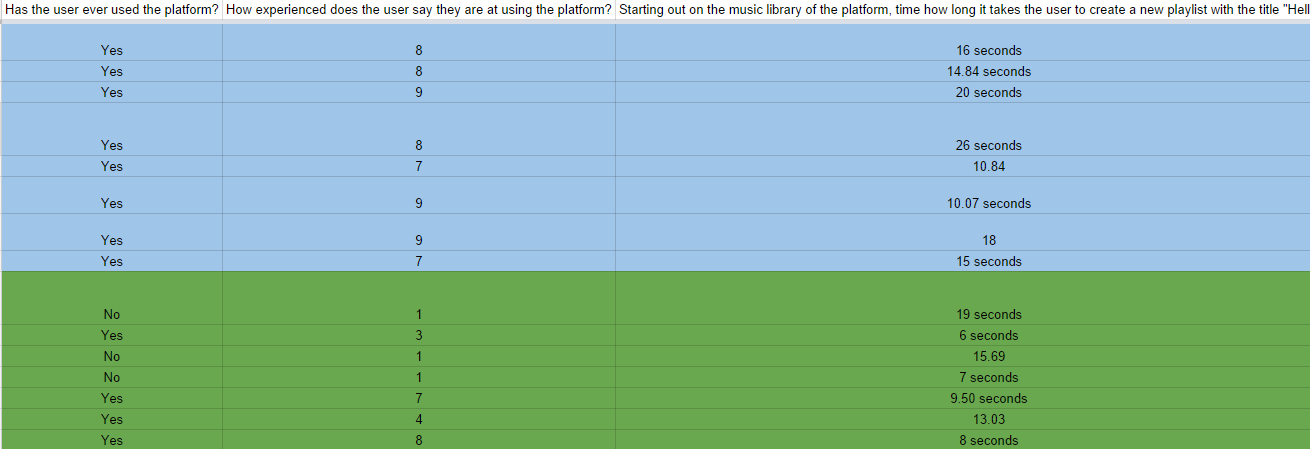
\includegraphics[width=0.6\textwidth]{tasks1.PNG}
\caption{\label{task:tasks1.1}Blue=iTunes  Green=Spotify}
\end{figure}
\begin{figure}[H]
\centering
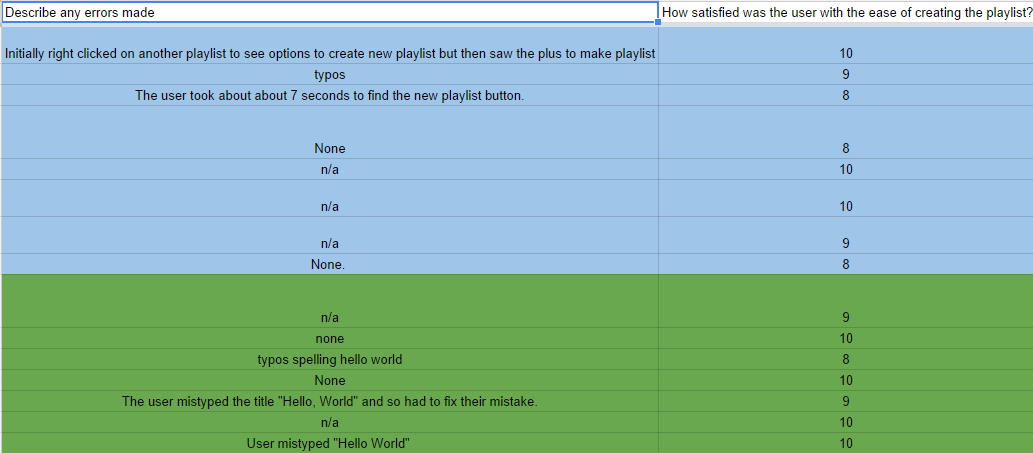
\includegraphics[width=0.6\textwidth]{tasks2.PNG}
\caption{\label{task:tasks1.2}Blue=iTunes  Green=Spotify}
\end{figure}
\begin{figure}[H]
\centering
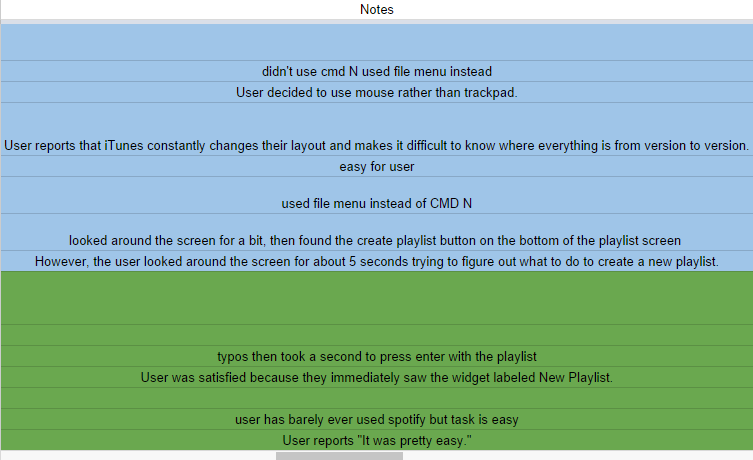
\includegraphics[width=0.6\textwidth]{tasks3.PNG}
\caption{\label{task:tasks1.3}Blue=iTunes  Green=Spotify}
\end{figure}

\subsection{Task 1}


As shown below, our results indicated that for the first task the timing, which was used to measure efficiency, iTunes was on average much slower to complete the task of creating a playlist titled "Hello World" than Spotify was. This was the most important of the measurements we focused on, as well as the errors, which occurred less for those using iTunes than those using Spotify by a small margin.The last measurement which we compared amongst the two was satisfaction, which was as close as the errors comparison was between the two platforms, yet Spotify performed better in this measure as well. Overall for this task we determined Spotify to be the superior platform. 

\subsection{Task 2}

\begin{figure}[H]
\centering
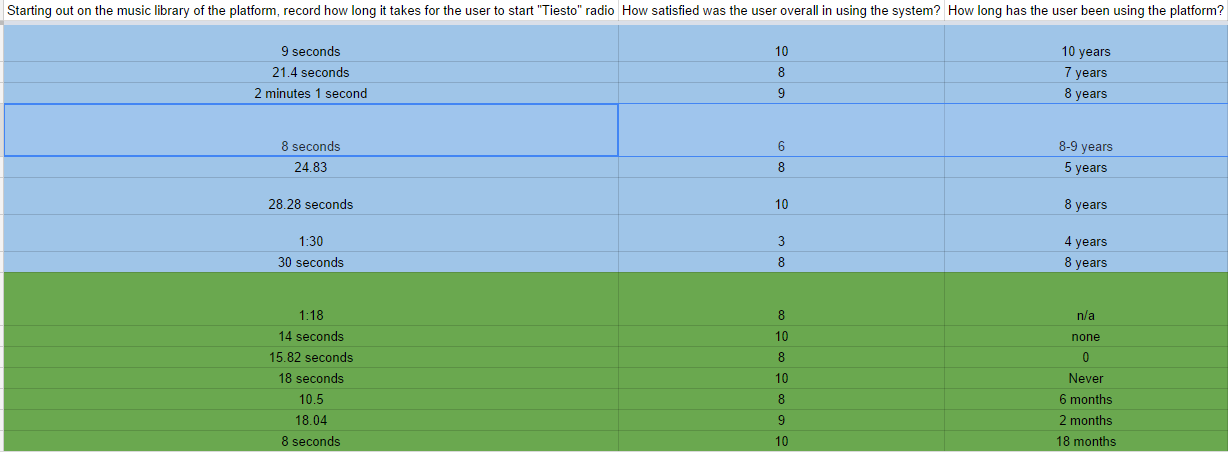
\includegraphics[width=0.6\textwidth]{task2_1.PNG}
\caption{\label{task:task2.1}Blue=iTunes  Green=Spotify}
\end{figure}
\begin{figure}[H]
\centering
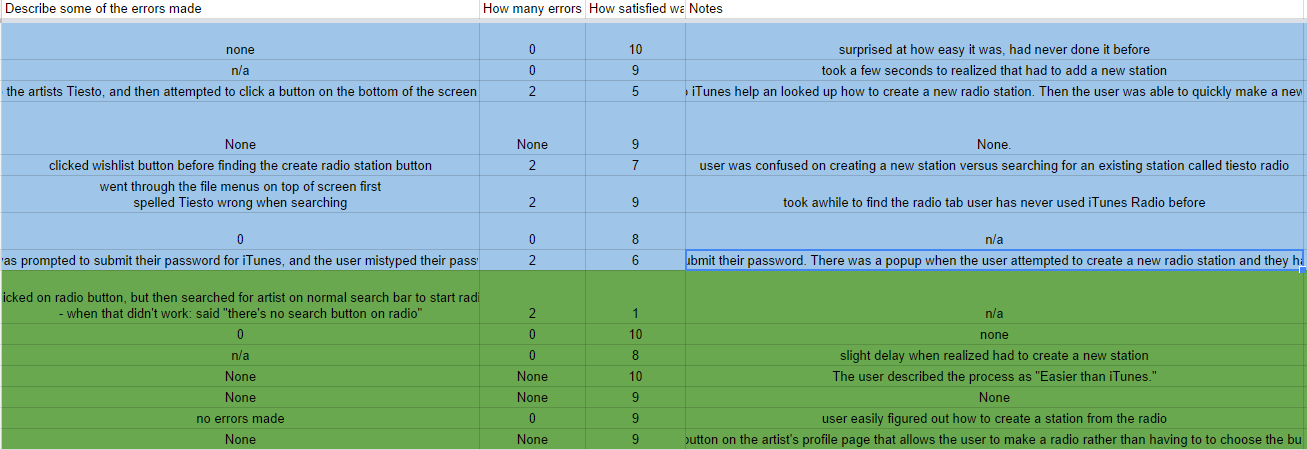
\includegraphics[width=0.6\textwidth]{task2_2.PNG}
\caption{\label{task:task2.2}Blue=iTunes  Green=Spotify}
\end{figure}

For our second task, which was for the user to create a radio station for the artist "Tiesto", we again found Spotify to be the superior platform. For our most important task of efficiency, we found the efficiency comparison between the two platforms to have a larger deficit than the first task, in Spotify's favor. OUr error total for this task was quite lopsided, with fewer errors occuring while the users were on Spotify. The satisfaction rating follows the same pattern as the other two measures we chose to focus on, with Spotify receiving higher ratings from its users than iTunes.


\subsection{Task 3}

\begin{figure}[H]
\centering
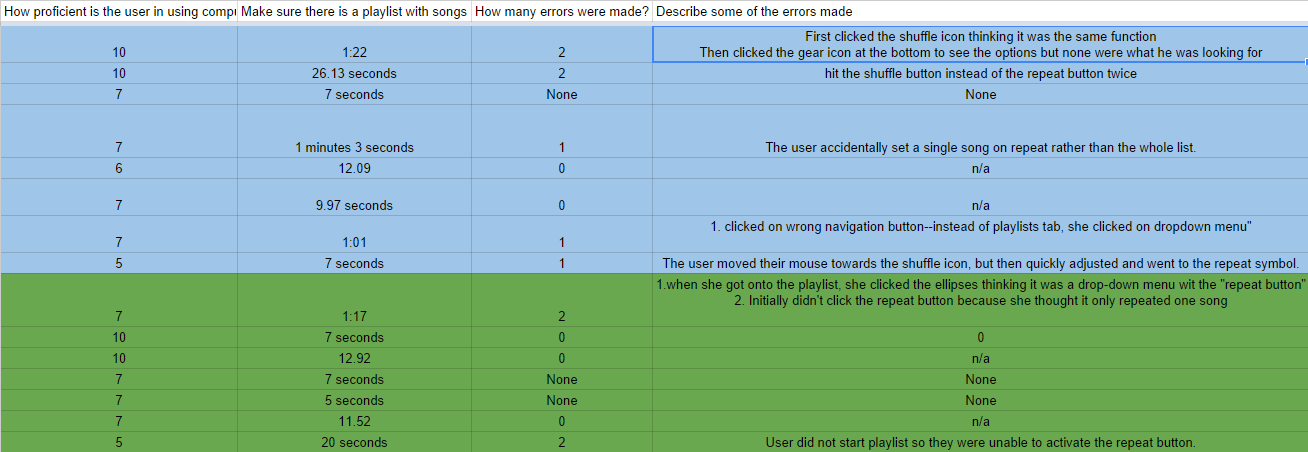
\includegraphics[width=0.6\textwidth]{task3_1.PNG}
\caption{\label{task:task3.1}Blue=iTunes  Green=Spotify}
\end{figure}
\begin{figure}[H]
\centering
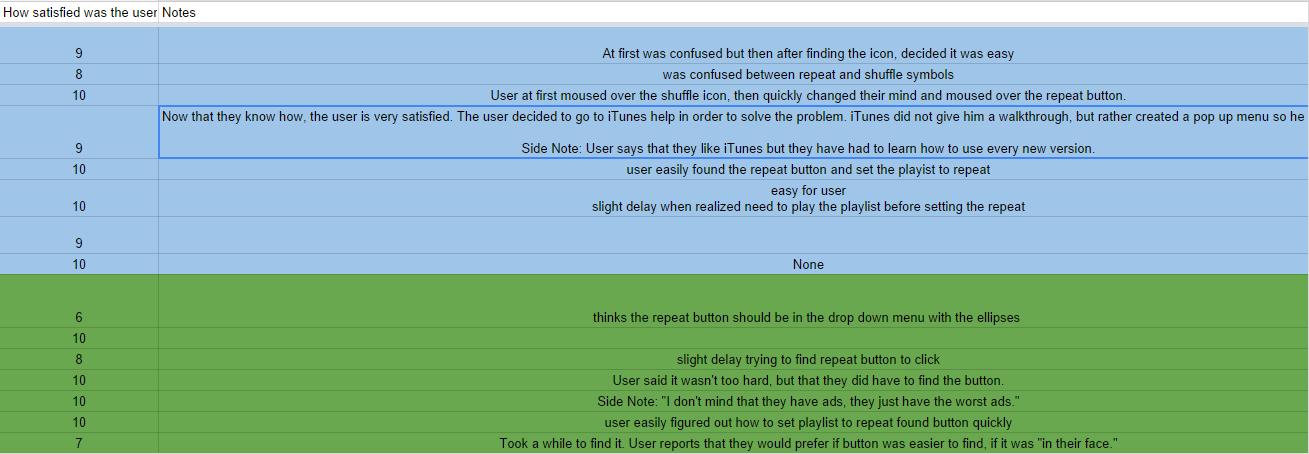
\includegraphics[width=0.6\textwidth]{task3_2.PNG}
\caption{\label{task:task3.2}Blue=iTunes  Green=Spotify}
\end{figure}

As for our third and final task, we found the results to be just as conclusive as the other two. For our most heavily weighted measure, efficiency, Spotify was more efficient in regard to the average time it took the users to complete the task. When we measured the erros for this task, there were more erros for iTunes again and less errors for Spotify. When we get to satisfaction, the motif of higher satisfaction for Spotify returns and we see that Spotify does indeed measure better than iTunes as a superior platform for these usability measurements.



\section{Heuristic Evaluation}

After determining Spotify to be the superior platform based on our field study results and how they can be judged using our weighted usability measurements system we decided to analyze why we believe each platform performed the way that they did for each task. Befor we begin I would like to show a screenshot of both platforms for future reference.

\begin{figure}[H]
\centering
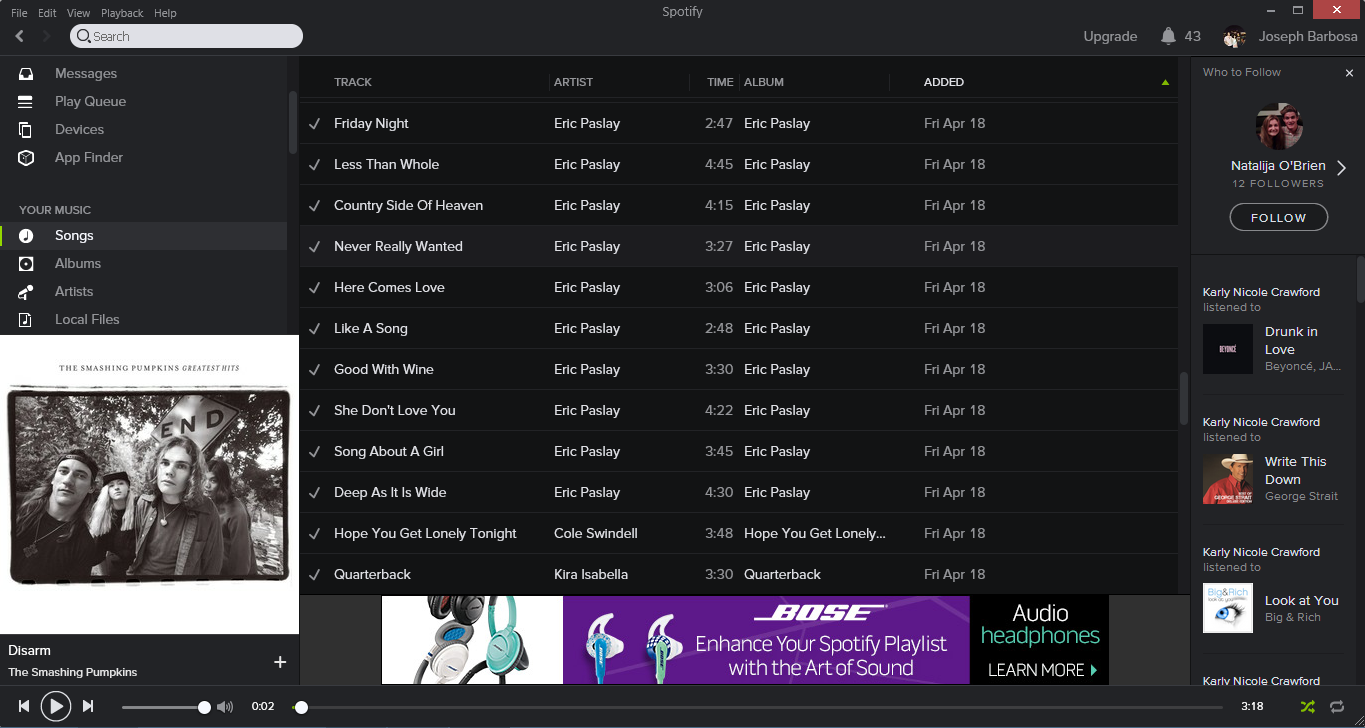
\includegraphics[width=0.6\textwidth]{spotify.PNG}
\caption{\label{task:spotify}Spotify}
\end{figure}
\begin{figure}[H]
\centering
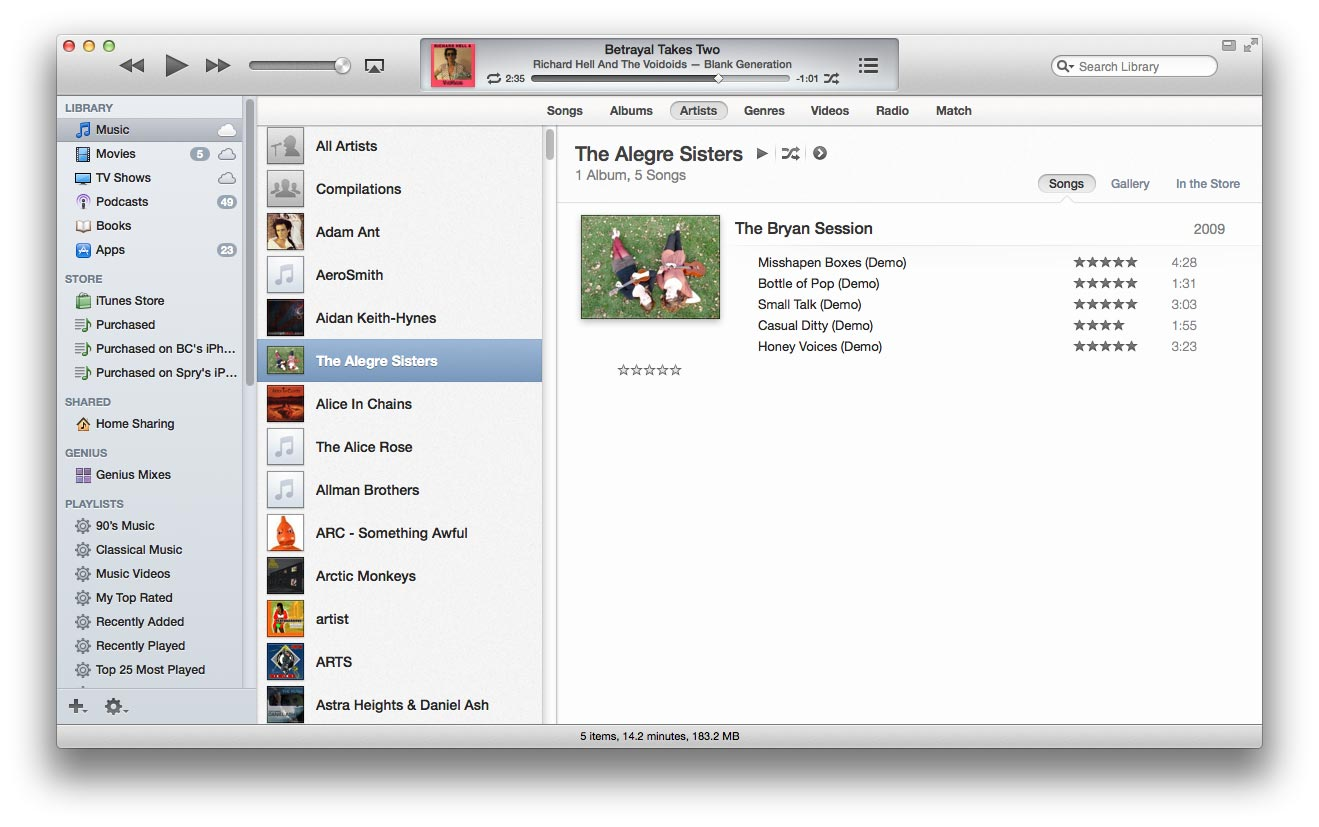
\includegraphics[width=0.6\textwidth]{itunes.jpg}
\caption{\label{task:iTunes}iTunes}
\end{figure}

For our first task, going over Spotify's guidelines documents versus Apple's guidelines documents many differneces were evident as to why Spotify tested better. Apple uses tab bars, controls, and a side panel to interact with the user for their navigation and destinationa; purposes. Yet for this task, Apple failed to make the task as easy as possible for their user and lost functionality by having a button as their control to complete the action of creating a new playlist, which you must click before viewing a list of possible actions which include making a new playlist. This may have seemed most effective for the programmers since it allows users to go to the same place in the application for creating multiple things yet it takes more time for each task. Naming was the same for both processes, a simple click on the location of the playlist in the left hand side bar allowed the user to change the name. Spotify, however, adheres  directly to their guidelines documens for functionality and makes a control for their new playlist a simple control in the left hand side bar with a title stating what the button itself does so as not to confuse the user and save them time and stress in figuring out how to make a new playlist. 

The second task was a bit different, considering the layout of iTunes and Spotify. Itunes believes in the tab bar and side navigation bar as well as viewports for its layout whereas Spotify has one main side bar for navigation, a main central screen as a viewport and seperate side bars to do different functions. This may seem overwhelming but it is organized and is less confusing as it shows the users everything in an easy to navigate manner. In order to start a radio from the main library in iTunes, one must select the radio tab on the tab bar in iTunes, which some users missed, and then there were extra steps involved in locating where to input the artist and such. Whereas for Spotify the radio option was clearly labeled within the main navigation bar on the left hand side, which is an infinite scroll side bar, and it immediately allows for the user to input what radio they wish to start. This was a key difference amongst the two. They both did comply to their guidelines, yet one proved to be more effective and functional than the other.

Our last task showed just how well each platform stuck to their independent guidelines documents. In the apple application documents, the playbar and icon guidelines are set such that they are grouped together and allow the user to easiy select their desired option and each control would do its proper function. Yet the placement of these controls was not clearly stated and this led to confusion for the users while completing this task. For itunes, while a song is playing, as you can see in the screenshot, the shuffle icon appears miniscule in the playbar on the left hand side of the scrub slider for the song and the repeat is on the right hand side, seperated and consfusing to the user. This led to many users not being able to locate the control for repeat easily and this led to a decrease in efficeiency, more erros, and lower staisfaction rating. Spotify, however did comply with its guildeines and make the controls in the playbar appear next to each other and large enought that the user can clearly see which button they are choosing. This led to higher satisfaction ratings, less errors, and more efficient times.

Not only did the field tests prove that Spotify was the superior platform due to the results when analyzed using our weighted system of usability measurements, it also was proven in comparison to how the platforms comply to their guideines documents and how they focus on functionality for the user and how they organize their layout and navigation. This was a key point of comparison that can be used to measure the difference between the two platforms.

\begin{thebibliography}{1}

\bibitem{spotify} Spotify {\em https://developer.spotify.com/technologies/apps/guidelines/design/}  2014.

\bibitem{itunes}  Apple Inc. {\em https://developer.apple.com/library/ios/documentation/userexperience/conceptual/mobilehig/}
2014.
\end{thebibliography}

\end{document}